\scanpage{9}
1) \uline{Sets with permutation} $(E,u)\Longleftrightarrow\mathbb{Z}$-sets.

Classification : family of cardinals associated with the subgroups of $\mathbb{Z}$
\[
=\text{family of cardinals}\quad
\begin{tikzpicture}[baseline=-1ex]
\draw[gray!55,line width=.2pt] (0,.08)--(.08,-.10);
\draw[gray!80,line width=.35pt] (.08,-.10)--(.25,.08);
\node[inner sep=0pt] at (.34,.08) {$\unsure{\phantom{x}}$};
\end{tikzpicture}\quad(a_i)_{i\in\mathbb{N}}
\]

\[
E\ \text{finite}\Longleftrightarrow
\underbrace{n_{0}=0}_{\substack{\text{finite}\\\text{orbits}}}
\ \text{and}\quad
\underbrace{\text{the } n_{i}\ \text{finite}}_{\substack{\text{finite number of}\\\text{orbits of}\\\text{cardinality } i\in\mathbb{N}\\\text{given}}},
\quad\underbrace{\text{zero except for a finite number}}_{\text{finite number of orbits}}
\]

$u$ transitive ($\Longleftrightarrow u$ defines on $E$ a circular order) $\Leftrightarrow$ all the $n_{i}$ except at most one are zero

\uline{Corollary} The classes of elements of $\unsure{\mathfrak{S}|\mathscr{S}}_{n}$ modulo conjugation correspond $1$-$1$\par
\noindent\begin{tabular}{@{}|@{\hspace{.6em}}p{\dimexpr\linewidth-1em\relax}@{}}
to the ``partitions'' of $n$, i.e. to the families of integers $(c_{i})_{1\leq i\leq n}$ such that
\[
\makebox[\linewidth][l]{$\displaystyle\sum i c_{i}=n$}
\]
\end{tabular}

\diagram{\resizebox{\linewidth}{!}{\begingroup\setlength{\arraycolsep}{2.5pt}\(\begin{array}{ll l|ll l}
\mathfrak{S}_{2}:&2\ \text{\unsure{classes|class}}&1,\sigma_{12}&\unsure{\mathfrak{A}|\mathscr{A}}_{2}:&1\ \text{class}&1\\
\mathfrak{S}_{3}:&3\ \text{classes}&1,\sigma_{12},\sigma_{123}&\mathfrak{A}_{3}:&3\ {-}&1,\sigma_{123},\sigma_{321}\\
\mathfrak{S}_{4}:&5\ \text{classes}&1,\sigma_{12},\sigma_{12}\sigma_{34},\sigma_{123},\sigma_{1234}
&\mathfrak{A}_{4}:&\multicolumn{2}{l}{\tikz[baseline=(entry.base)]{
  \node[inner sep=1.5pt] (entry) {$\deleted{\unsure{1|i},\sigma_{\unsure{12|13}}\sigma_{\unsure{34|24}},\sigma_{\unsure{1234|4234}}}$};
  \draw[rounded corners=2.5pt] ([xshift=-2em,yshift=1.5pt]entry.north east)
    -- ([xshift=-2em]entry.north east) -- (entry.north west) -- (entry.south west)
    -- ([xshift=-1.65em]entry.south east) -- ([xshift=-1.65em,yshift=-1.5pt]entry.south east);
}}\\
\mathfrak{S}_{5}:&?&&&&
\end{array}\)\endgroup}}

2) \uline{Correction} The oriented contours correspond to the sets with permutation $(E,u)$ such that $u$ does \uline{not have a fixed point} (for we do not want a polygon with $1$ side, in graphs !)

3) $\frac{1}{2}$ direct product of groups

\diagram{\begin{tikzcd}[ampersand replacement=\&,column sep=small]
\text{giving}\&[-1ex]1 \arrow[r,dash] \& \mathbb{Z}\arrow[r,dash,"i"] \& G\arrow[r,dash,"p"] \& \Gamma\arrow[l,bend left=24,"q"']\arrow[r,dash] \& 1q \&[-1ex] \unsure{p|q}qp=\operatorname{id}_{\Gamma}\quad\unsure{q|p}
\end{tikzcd}}
(exact sequence, with $q$ a homomorphism of \unsure{groups|groups})

amounts to giving
\diagram{\begin{tikzcd}[ampersand replacement=\&,column sep=small,row sep=0pt]
1\arrow[r,dash] \& Z\arrow[r,dash] \& G\arrow[r] \& \Gamma\arrow[r,dash] \& 1 \& p\mid\Gamma'\simeq\deleted{\unsure{\mathrm{isomorphism}|\mathrm{is}}}\Gamma\ \text{\unsure{isomorphism|is}}\\
\& \& \rotatebox{90}{$\subset$} \\
\& \& \Gamma'
\end{tikzcd}}

or to giving \unsure{groups|groups} $Z,\Gamma$ with action of $\Gamma$ on $Z$
\[
\Gamma\longrightarrow\operatorname{Aut}_{\mathrm{gr}}(Z)
\]

composition law on $G=\mathbb{Z}\times\Gamma$

% left margin note, slanted; the diagonal divider is retained
\reversemarginpar
\margin{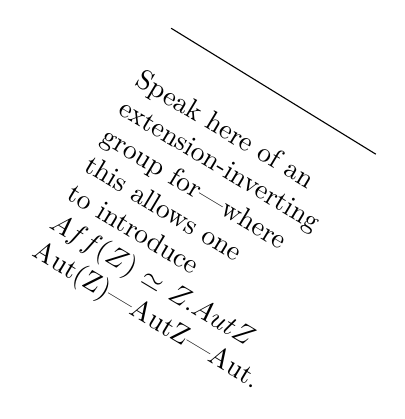
\begin{tikzpicture}
\draw (0,0.4)--(2.6,-1.2);
\node[anchor=north west,rotate=-31,align=left,text width=3.2cm,inner sep=0pt] at (-0.35,-0.1)
{\unsure{Speak} here of an extension-inverting group \unsure{for|where} this allows one to introduce $\operatorname{Aff}(Z)\simeq Z.\operatorname{Aut}Z$ \deleted{\unsure{Aut(Z)|AutZ|Aut}}.};
\end{tikzpicture}}
\normalmarginpar

\[
\begin{aligned}
&\deleted{(\gamma,z)(\gamma',z')=(\gamma\gamma',\operatorname{int}(\gamma')^{-1}(z).z')}\\
&(z,\gamma)(\unsure{z'|{\mathcal Z}'},\gamma')=(z\operatorname{int}(\gamma)(z'),\gamma\gamma')
\end{aligned}
\]

% Lower-right note with its oblique divider and the short adjacent stroke.
\margin{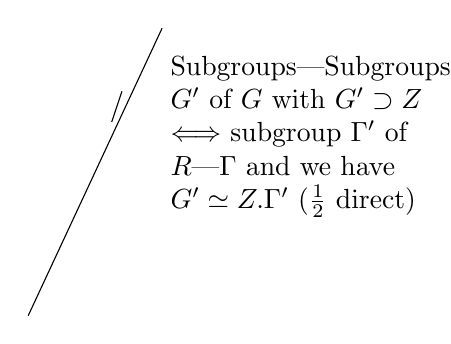
\begin{tikzpicture}
\draw (0,-3.5)--(1.7,0.15);
\draw (1.06,-1.04)--(1.19,-0.65);
\node[anchor=north west,align=left,text width=3.2cm,inner sep=0pt] at (1.8,-0.2)
{\unsure{Subgroups|Subgroups} $G'$ of $G$ with $G'\supset Z$ $\Longleftrightarrow$ subgroup $\Gamma'$ of \deleted{\unsure{$R$|$\Gamma$}} and we have $G'\simeq\mathbb{Z}.\Gamma'$ ($\frac{1}{2}$ direct)};
\end{tikzpicture}}
% archive sheet number: 8
